% Kopfzeile beim Kapitelanfang:
\fancypagestyle{plain}{
%Kopfzeile links bzw. innen
\fancyhead[L]{\Large Vorlesung 25 (20.01.2013)}
%Kopfzeile rechts bzw. außen
\fancyhead[R]{}}
%Kopfzeile links bzw. innen
\fancyhead[L]{\Large Vorlesung 25 (20.01.2014)}
%Kopfzeile rechts bzw. außen
\fancyhead[R]{}
% **************************************************
\enk{
\setcounter{enumi}{1}
\item $\sum_{n=0}^\infty z^n$ (geom. Reihe); $\sum_{n=1}^\infty \frac{z^n}{n}$; $\sum_{n=1}^\infty \frac{z^n}{n^2}$\\
Konvergenzradius: Stets $R=1$ mit (1)\nl
z.B. 3. Reihe: $c_n = \frac{1}{n^n} \Ra \lim_{n \to \infty} \left|\frac{c_{n+1}}{c_n}\right| = \lim_{n \to \infty} \frac{n^2}{(n+1)^n} = 1 \Ra R=1$\\
1. Reihe: divergiert $\forall z \in \C$ mit $|z|=1$ (dann $(z^n)$ keine Nullfolge)\\
2. Reihe: divergiert für $z=1$ (Harm. Reihe), konvergiert für $z=-1$ (alt. Harm. Reihe)\\
3. Reihe: $|z|=1 \Ra \left|\frac{z^n}{n^2}\right| = \frac{1}{n^2} \sum_{n=1}^\infty \frac{1}{n^2} < \infty \Ra \sum_{n=1}^\infty \frac{z^n}{n^2}$ konvergiert $\forall z$ mit $|z|=1$
}

\subsection*{Fazit}
Am Rand des Konvergenzkreises ist keine allgemeingültige Aussage möglich!

\subsection*{Bemerkung}
Für allgemeine Potenzreihen $\sum c_n (z-a)^n$ hat man eine konvergente Kreisscheibe $K_R(a) = \{z \in \C: |z-a| < R\}$\\
$R=$ Konvergenzradius von $\sum_{n=0}^\infty c_n z^n$\nl
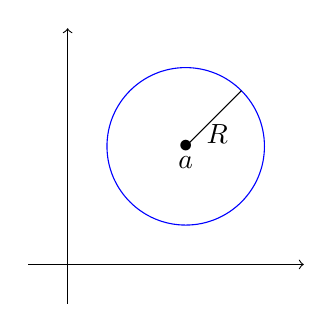
\begin{tikzpicture}
\draw[->] (-0.5,0)--(3,0);
\draw[->] (0,-0.5)--(0,3);
\draw[color=blue] (1.5,1.5) circle (1);
\draw (1.5,1.5) node {$\bullet$} node[below] {$a$};
\draw (1.5,1.5)--(2.20710678,2.20710678);
\draw (1.9,1.9) node[below] {$R$};
\end{tikzpicture}

\section{Satz: Ableitung von Potenzreihen}\label{13.14}
Sei $f(x)=\sum_{n=0}^\infty c_n (x-a)^n$ eine Potenzreihe mit $c_n,a \in \R$ und Konvergenzradius $R>0$, betrachtet für $x \in \R$.\nl
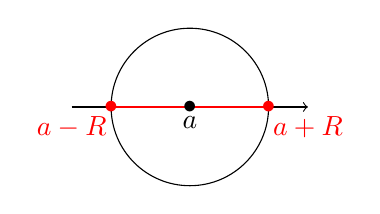
\begin{tikzpicture}
\draw[->] (-1.5,0)--(1.5,0);
\draw (0,0) circle (1);
\draw[color=red] (-1,0) node {$\bullet$};
\draw[color=red] (1,0) node {$\bullet$};
\draw[color=red] (-1.5,0) node[below] {$a-R$};
\draw[color=red] (1.5 ,0) node[below] {$a+R$};
\draw[color=red] (-1,0)--(1,0);
\draw (0,0) node {$\bullet$} node[below] {$a$};
\end{tikzpicture}\nl
\en{
\item[$\Ra$ (1)] Die gliedweise differenzierte Potenzreihe\\
$\sum_{n=1}^\infty n c_n (x-a)^{n-1}$ hat ebenfalls Konvergenzradius $R$
\item[(2)] $f$ ist stetig differenzierbar auf dem offenen Intervall $(a-R,a+R)$, $f'(x)=\sum_{n=1}^\infty n c_n (x-a)^{n-1}$ ohne Beweis
}
Iteration $\Ra f$ ist beliebig oft differenzierbar auf $(a-R,a+R)$ und darf jeweils gliedweise differenziert werden.

\subsection*{Beispiel}
$L(x) := \sum_{n=1}^\infty \frac{(-1)^{n-1}}{n} x^n$ "`\underline{Logarithmusreihe}"'\\
Konvergenzradius: $R=1$ (mit Krit. (1))\\
Satz \ref{13.14} $\Ra L$ ist stetig differenzierbar auf $(-1,1)$\\
mit $L'(x) = \sum_{n=1}^\infty (-1)^{n-1} x^{n-1} = \sum_{n=0}^\infty (-x)^n = \frac{1}{1+x}$ (geom. Reihe) \emph{(i)}\\
Andererseits: $\frac{d}{dx} \ln\underbrace{(1+x)}_{>0} = \frac{1}{1+x}$ \emph{(ii)}\nl
\emph{(i)}+\emph{(ii)} $\underset{\text{Satz \ref{11.13}}}{\Ra} L(x)-\ln(1+x) = c =$ konst. auf $(-1,1)$\\
Bestimme $c$: Setze $x=0$: $c=\underbrace{L(0)}_{=0}-\underbrace{\ln 1}_{=0}=0$\\
$\Ra \forall x \in (-1,1)$: \fbox{$\ln(1+x) = \sum_{n=1}^\infty \frac{(-1)^{n-1}}{n} x^n$} (*)\nl
\begin{tikzpicture}
\draw (-3,0)--(3,0);
\draw (-2,0) node {$($} node[below] {$-1$};
\draw (2,0) node {$)$} node[below] {$1$};
\draw (0,0) node {$|$} node[below] {$0$};
\draw[color=red] (-1.75,0) node {$|$};
\draw[color=red] (1.75,0) node {$|$};
\draw[color=red] (-1.75,0)--(1.75,0);
\draw (0,0.5)--(2,0.5) node {$|$};
\draw (0,0.5) node {$|$};
\end{tikzpicture}\nl
Die Logarithmusreihe $L(x)$ konvergiert nach Leibnizkriterium auch für $x=1$: $L(1)=\sum_{n=1}^\infty \frac{(-1)^{n-1}}{n} = 1 - \frac{1}{2} + \frac{1}{3} - \frac{1}{4} + \ldots$\\
Vermutung: Die Reihenentwicklung (*) gilt auch noch für $x=1$, das heißt $\ln 2 = \sum_{n=1}^\infty \frac{(-1)^{n-1}}{n}$.

\subsection*{Beweis}
In der Übung.

\chapter{Integration}\label{P14}
\begin{tikzpicture}
\draw[->] (-2.5,0)--(2.5,0);
\draw[dashed,domain=-2.5:-2] plot (\x, {-1*sin(deg(\x))});
\draw[dashed,domain=2:2.5] plot (\x, {-1*sin(deg(\x))});
\draw[color=blue,pattern=custom north west lines,hatchcolor=blue] (-2,0) -- plot [domain=-2:0] (\x, {-1*sin(deg(\x))}) -- (0,0) -- cycle;
\draw[color=blue] (-1.3,0.5) node {$F_1 > 0$};
\draw[color=red,pattern=custom north west lines,hatchcolor=red] (0,0) -- plot [domain=0:2] (\x, {-1*sin(deg(\x))}) -- (2,0) -- cycle;
\draw[color=red] (1.3,-0.5) node {$F_2 < 0$};
\draw (-2,0) node[below] {$a$};
\draw (2,0) node[above] {$b$};
\draw (0,0.5) node {$\Gamma_f$};
\end{tikzpicture}\nl
Idee: $\int_a^b f(x) dx=$ Fläche zwischen $\Gamma_f$ und der x-Achse $=F_1+F_2$\\
Falls $f$ stückweise konst.: jeweils Grundlinie $\cdot$ Höhe\nl
\begin{tikzpicture}
\draw[->] (-3.5,0)--(3.5,0);
\draw[color=blue] (-3,2)--(-1,2);
\draw[dashed] (-3,2)--(-3,0) node[below] {$a$};
\draw[dashed] (-1,2)--(-1,0);
\draw (-2,1) node {$+$};
\draw[color=blue] (-1,-1)--(1,-1);
\draw[dashed] (-1,-1)--(-1,0);
\draw[dashed] (1,-1)--(1,0);
\draw (0,-0.5) node {$-$};
\draw[color=blue] (1,2)--(3,2);
\draw[dashed] (1,2)--(1,0);
\draw[dashed] (3,2)--(3,0) node[below] {$b$};
\draw (2,1) node {$+$};
\end{tikzpicture}

\section{Definition: Integral von Treppenfunktionen}\label{14.1}
$f: [a,b] \to \R$ heißt \underline{Treppenfunktion} $:\Lra \exists$ Unterteilung\\
$a=x_0 < x_1 < \ldots < x_n = b$, so dass\\
$f \mid_{(x_{n-1}, x_k)}=$ konst. $=c_k \forall k=1,\ldots,n$\nl
Setze: $\int_a^b f(x) dx := \sum_{k=1}^n c_k (x_k - x_{k-1})$ \underline{Integral von $f$ über $[a,b]$}\\
$T[a,b] := \{f: [a,b] \to \R \text{ Treppenfunktion}\}$\nl
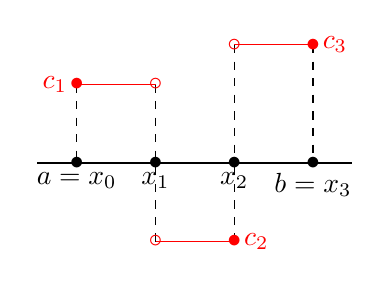
\begin{tikzpicture}
\draw (-0.5,0)--(3.5,0);
\draw (0,0) node {$\bullet$} node[below] {$a=x_0$};
\draw (1,0) node {$\bullet$} node[below] {$x_1$};
\draw (2,0) node {$\bullet$} node[below] {$x_2$};
\draw (3,0) node {$\bullet$} node[below] {$b=x_3$};
\draw[dashed] (0,1)--(0,0) (1,1)--(1,0) (1,-1)--(1,0) (2,-1)--(2,0) (2,1.5)--(2,0) (3,1.5)--(3,0);
\draw[color=red] (0,1) node {$\bullet$} node[left] {$c_1$} --(1,1) node {$\circ$};
\draw[color=red] (1,-1) node {$\circ$} --(2,-1) node {$\bullet$} node[right] {$c_2$};
\draw[color=red] (2,1.5) node {$\circ$} --(3,1.5) node {$\bullet$} node[right] {$c_3$};
\end{tikzpicture}

\newpage

\subsection*{Beachte}
\enk{
\item $\int_a^b fdx$ ist unabhängig von den Werten von $f$ an den Teilpunkten und ändert sich nicht bei Einfügen zusätzlicher Teilpunkte (Verfeinerung der Unterteilung)\nl
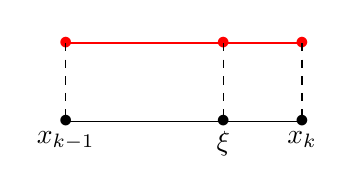
\begin{tikzpicture}
\draw (0,0)--(3,0);
\draw[color=red] (0,1) node {$\bullet$} --(2,1) node {$\bullet$} --(3,1) node {$\bullet$};
\draw[dashed] (0,1)--(0,0) (2,1)--(2,0) (3,1)--(3,0);
\draw (0,0) node {$\bullet$} node[below] {$x_{k-1}$};
\draw (2,0) node {$\bullet$} node[below] {$\xi$};
\draw (3,0) node {$\bullet$} node[below] {$x_k$};
\end{tikzpicture}
\item $f,g \in T[a,b], \lambda \in \R \Ra \lambda f, |f| \in T[a,b]$ (klar)\\
$f+g \in T[a,b]$, denn: $f$ Treppenfunktion zu Unterteilung $Z = \{x_0, \ldots, x_n\}$\\
$g$ ist Treppenfunktion zu Unterteilung $\{\tilde{x_0}(=x_0), \ldots, \tilde{x_n}\} = \tilde{Z}$\\
$\Ra f+g$ ist Treppenfunktion zu $Z \cup \tilde{Z}$
}

\section{Eigenschaften des Integrals von Treppenfunktionen}\label{14.2}
\en{
\item $\int_a^b (f+g) dx = \int_a^b fdx + \int_a^b gdx$ "`Linearität"' (1)
\item $\lambda \in \R \Ra \int_a^b (\lambda f) dx = \lambda \int_a^b fdx$ "`Linearität"' (2)
\item $f \le g$ auf $[a,b] \Ra \int_a^b fdx \le \int_a^b gdx$ "`Monotonie"'
\item $\left|\int_a^b fdx\right| \le \int_a^b |f| dx$
}

\subsection*{Beweis}
\en{
\item Wähle gemeinsame Unterteilung $\{a=x_0 < \ldots < x_n=b\}$ für $f,g$\\
$f \mid_{(x_{k-1},x_k)} = c_k, g \mid_{(x_{k-1},x_k)} = d_k$\\
$\Ra \int_a^b (f+g) dx = \sum_{k=1}^n (c_k+d_k)(x_k-x_{k-1}) = \int_a^b fdx + \int_a^b gdx$\\
}
Rest ähnlich. \qed

\section{Definition: Integration von Regelfunktionen}\label{14.3}
$f: [a,b] \to \R$ heißt \underline{Regelfunktion} $:\Lra \exists$ Folge $(\varphi_n)_{n \in \N}$ von Treppenfunktionen auf $[a,b]$\\
mit $\lim_{n \to \infty} ||f-\varphi_n||_{[a,b]} = 0$\nl
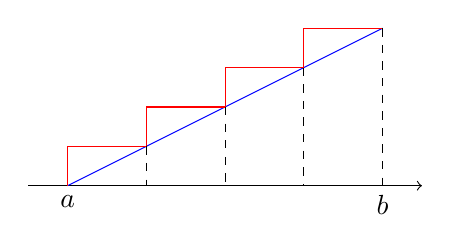
\begin{tikzpicture}
\draw[->] (-2.5,0)--(2.5,0);
\draw[color=blue] (-2,0)--(2,2);
\draw[color=red] (-2,0)--(-2,0.5)--(-1,0.5)--(-1,1)--(0,1)--(0,1.5)--(1,1.5)--(1,2)--(2,2);
\draw (-2,0) node[below] {$a$};
\draw[dashed] (-1,0.5)--(-1,0) (0,1)--(0,0) (1,1.5)--(1,0) (2,2)--(2,0) node[below] {$b$};
\end{tikzpicture}\nl
Abkürzung: $||f||_{[a,b]} =: ||f||$\nl
Also: $f$ Regelfunktion auf $[a,b] \Lra f$ gleichmäßig auf $[a,b]$ durch Treppenfunktion approximierbar\\
$R[a,b] := \{f: [a,b] \to \R \text{ Regelfunktion}\}$
% TODO: Graph (4)

\section{Definition: Folge von Treppenfunktionen}\label{14.4}
Sei $f \in R[a,b]$ und $(\varphi_n)_{n \in \N}$ \underline{Folge von Treppenfunktionen} auf $[a,b]$ mit $\lim_{n \to \infty} ||f-\varphi_n|| = 0$.\nl
Setze \fbox{$\int_a^b f(x) dx := \lim_{n \to \infty} \int_a^b \varphi_n(x) dx$}\nl
Diese Definition ist sinnvoll, denn:
\en{
\item Der Limes rechts existiert, da $\left(\int_a^b \varphi_n(x) dx\right)_{n \in \N}$ Cauchyfolge in $\R$, also konvergent.\\
Dazu: $\left|\int_a^b \varphi_n dx - \int_a^b \varphi_m dx\right| \underset{\text{\ref{14.2}}}{\le} \int_a^b \left|\underbrace{\varphi_n(x)-\varphi_m(x)}_{\le ||\varphi_n-\varphi_m||}\right| dx \underset{\text{Monotonie}}{\le} \int_a^b ||\varphi_n-\varphi_m|| dx$\\
$\underset{\text{Trick}}{=} (b-a) \cdot ||\varphi_n-\varphi_m|| \underset{\text{Dreiecksungl. für } ||\ldots||}{\le} (b-a) (||\varphi_n-f||+||f-\varphi_m||) < \eps \forall n,m \ge N_\eps$
\item Der Limes ist unabhängig von der Wahl der approx. Folge $(\varphi_n)$ (ohne Beweis, siehe z.B. Königsberger)
}

\subsection*{Beachte}
$f,g \in R[a,b], \lambda \in \R \Ra \lambda f, |f|, f+g \in R[a,b]$ (durch Approximieren mit Treppenfunktion)

\section{Satz: Eigenschaften des Integrals}\label{14.5}
Seien $f,g \in R[a,b]$.
\en{
\item $\int_a^b (f+g) dx = \int_a^b fdx + \int_a^b gdx$ "`Linearität"' (1)
\item $\int_a^b (\lambda f) dx = \lambda \cdot \int_a^b fdx$
\item $f \le g \Ra \int_a^b fdx \le \int_a^b gdx$ "`Monotonie"'
\item $|\int_a^b fdx| \le \int_a^b |f| dx \le (b-a) \cdot ||f||$
}

\subsection*{Beachte}
Jede Regelfunktion auf $[a,b]$ ist beschränkt.